\chapter{Gestión del proyecto}

Dentro de la ingeniería de software, una de las partes esenciales para la realización de proyectos considerados exitosos es la gestión de proyectos. La realización de una buena gestión no se puede considerar, ni mucho menos, una garantía de que el proyecto a gestionar vaya a resultar un éxito. Sin embargo, si elegimos ignorar o realizar una mala gestión de nuestro proyecto sí podremos considerar que nos encontraremos en una situación proclive para un proyecto fallido. Durante toda la extensión del ciclo de vida de nuestro proyecto se utilizará la gestión de proyectos como un método que nos ayudará a lograr la obtención de un producto final ajustado a todas las necesidades y restricciones presentes, sea cual sea la índole de las mismas (tiempo, costes, requisitos, etc.).

\bigskip

Dedicaremos este capítulo a definir y explicar la gestión de nuestro proyecto en todas sus partes. Se determinará y explicará el análisis de riesgos, la metodología de desarrollo empleada, la gestión de configuración, la planificación temporal y la estimación de costes.

\section{Gestión de riesgos}

Citando al PMBOK \cite{pmbok} la definición de riesgo es:

\begin{quote}
	\textit{
		“[...]un evento o condición incierta que, de producirse, tiene un efecto positivo o
		negativo en uno o más de los objetivos del proyecto, tales como el alcance, el cronograma, el costo y la calidad.”
	}
\end{quote}

Las causas de un riesgo pueden ser varias y diversas y, si este finalmente se diera, los impactos que puede producir también pueden ser numerosos. Dentro de las causas, su índole puede ser de tipos muy variados, desde un requisito mal especificado a una restricción que no existe pasando por supuestos que no se ajustan a realidad o fallos en procesos externos al proyecto. Si alguna de estas situaciones se produce podría haber un impacto relevante sobre los objetivos definidos previamente para el proyecto como lo serían el alcance, el coste, el cronograma o la calidad.

\bigskip

El impacto suele ser generalmente negativo aunque ocasionalmente puede ser beneficioso para el proyecto. En el proyecto al que se refiere esta memoria realizaremos una gestión de riesgos enfocada a los que tienen una naturaleza negativa y que por lo tanto podrían afectar a los objetivos de forma perjudicial. Una vez dicho esto, hay que considerar las diferentes estrategias que se pueden utilizar para abordar las amenazas o riesgos con impacto negativo en caso de materializarse y serán las siguientes:

\begin{itemize}
	
	\item \textbf{Evitar}: Siguiendo esta estrategia de respuesta el equipo del proyecto intentará eliminar la amenaza o proteger al proyecto del posible impacto de forma preventiva. Comúnmente implica modificar la planificación para evitar completamente la amenaza. 
	
	\item \textbf{Transferir}: Al transferir un riesgo el equipo traslada el impacto asociado al mismo a un tercero, librándose así de la responsabilidad de dar una respuesta si el riesgo se da. Suele incluir el pago de una prima de riesgo a la entidad que asumirá el impacto del mismo. 
	
	\item \textbf{Mitigar}: Mitigar un riesgo implica actuar para reducir o bien la probabilidad de un riesgo o bien el impacto que este tendría en el proyecto, llevando uno de estos aspectos o ambos a un umbral aceptable. Habitualmente es más efectivo realizar acciones preventivas que intentar lidiar con el riesgo una vez que ha ocurrido. 
	
	\item \textbf{Aceptar}: Si el equipo decide reconocer el riesgo y no hacer nada al respecto a menos que este se materialice la estrategia que se está utilizando es la de aceptar dicho riesgo. Esta aproximación se suele utilizar si no es posible o rentable utilizar alguna de las otras estrategias. Esto puede implicar no realizar ninguna acción si el riesgo ocurra (estrategia pasiva) o establecer una reserva para contingencias que pueda aportar los recursos, tiempo o dinero necesarios para gestionar el riesgo (estrategia activa).
	
\end{itemize}

Dada la índole del proyecto y considerando el hecho de que solo hay un trabajador encargado del mismo se intentará evitar la transferencia de un riesgo al ser esta estrategia propensa a generar costes adicionales. Por razones similares, la aceptación de un riesgo se deberá considerar única y exclusivamente si ninguna de las otras estrategias es aplicable.

Para realizar un buen análisis de riesgos se debe comenzar por una identificación de la mayor cantidad de riesgos posible dentro de unos límites lógicos para luego analizar la importancia de cada uno teniendo en cuenta su probabilidad e impacto. Finalmente se deberán establecer estrategias a seguir en caso de que los riesgos se den, priorizando los más importantes en caso de que no sea posible gestionarlos todos.

\subsection{Especificación de riesgos}

Se dedicará este apartado a mostrar las especificaciones formales de los riesgos que contendrán su descripción, probabilidad, impacto y los planes diseñados para cada uno de ellos. La probabilidad\footnote{indicada como $p$ dentro de la tabla}  e impacto\footnote{indicada como $i$ dentro de la tabla} podrán tomar los valores definidos en el Cuadro \ref{tab:probabilidad_impacto}. El identificador utilizado para los riesgos tendrá la forma RSK\footnote{En referencia a \textit{risk}, riesgo en inglés}-\textit{N}


\begin{table}
	\begin{center}
		\caption{Valores posibles de probabilidad e impacto}
		\label{tab:probabilidad_impacto}
	\begin{tabular}{ | c | c | c | } 
		\hline
		
		\textbf{Calificativo} &
		\textbf{Probabilidad}&
		\textbf{Impacto}\\
		
		\hline
		Muy Bajo 
		&
		$p<0,10$
		&
		$i<0,10$
		\\ 
		
		\hline
		Bajo 
		&
		$0,10<=p<0,30$
		&
		$0,10<=i<0,20$
		\\ 
		
		\hline
		Moderado 
		&
		$0,30<=p<0,50$
		&
		$0,20<=i<0,40$
		\\ 
		
		\hline
		Alto 
		&
		$0,50<=p<0,70$
		&
		$0,40<=i<0,80$
		\\ 
		
		\hline
		Muy Alto 
		&
		$0,70<=p$
		&
		$0,80<=i$
		\\ 
		
		
		\hline
	\end{tabular}
\end{center}
\end{table}

\newcounter{contador_riesgos}
\setcounter{contador_riesgos}{1}

\begin{center}
	\begin{tabular}{ | p{5.6cm} | p{8.5cm} | } 
		\hline
		
		\textbf{ID} & RSK-\arabic{contador_riesgos}
		\refstepcounter{contador_riesgos} \\
		
		\hline 
		\textbf{Nombre} &
		Retraso en la planificación\\ 
		
		\hline
		\textbf{Descripción} & 
		Se debe contemplar la posibilidad de que ocurran retrasos en la planificación dada la inexperiencia del desarrollador a la hora de trabajar en un proyecto de esta envergadura y con algunas de las tecnologías a utilizar.\\
		
		\hline 
		\textbf{Probabilidad de ocurrencia} &
		Alta\\
		
		\hline 
		\textbf{Impacto} &
		Muy Alto\\
		
		\hline 
		\textbf{Plan de Prevención} &
		\textbf{Mitigar}: Realizar reuniones periódicas con los tutores del proyecto para resolver dudas y ver el avance del mismo.\\
		
		\hline 
		\textbf{Plan de Contingencia} &
		\textbf{Aceptar}:Redefinir el alcance del proyecto volviendo a evaluar los requisitos para priorizar los mas necesarios dejando los no vitales fuera del proyecto.\\
		
	
		\hline
	\end{tabular}
\end{center}

\begin{center}
	\begin{tabular}{ | p{5.6cm} | p{8.5cm} | } 
		\hline
		
		\textbf{ID} & RSK-\arabic{contador_riesgos}
		\refstepcounter{contador_riesgos} \\
		
		\hline 
		\textbf{Nombre} &
		Cambio en los requisitos\\ 
		
		\hline
		\textbf{Descripción} & 
		Es posible que una vez avanzado el proyecto se considere que algunos de requisitos necesitan ser añadidos, modificados o eliminados, especialmente dado que se dedicará cierta parte del proyecto a investigar la utilidad de técnicas de inteligencia artificial sobre las cuales se desconoce si serán de utilidad.\\
		
		\hline 
		\textbf{Probabilidad de ocurrencia} &
		Alta\\
		
		\hline 
		\textbf{Impacto} &
		Alto\\
		
		\hline 
		\textbf{Plan de Prevención} &
		\textbf{Mitigar}: Realizar un diseño de la aplicación de la forma más modular posible para evitar grandes refactorizaciones a la hora de hacer modificaciones importantes.\\
		
		\hline 
		\textbf{Plan de Prevención 2} &
		\textbf{Mitigar}: Utilizar una metodología de trabajo ágil que sea capaz de aceptar y soportar cambios sustanciales en los requisitos del proyecto.\\
		
		
		\hline
	\end{tabular}
\end{center}

\begin{center}
	\begin{tabular}{ | p{5.6cm} | p{8.5cm} | } 
		\hline
		
		\textbf{ID} & RSK-\arabic{contador_riesgos}
		\refstepcounter{contador_riesgos} \\
		
		\hline 
		\textbf{Nombre} &
		Falta de comprensión de conceptos\\ 
		
		\hline
		\textbf{Descripción} & 
		Puede ocurrir que el desarrollador no esté tan familiarizado con los conceptos relacionados con inteligencia artificial como es necesario para la realización del proyecto, dificultando así la implementación correcta de cualquiera de sus técnicas.\\
		
		\hline 
		\textbf{Probabilidad de ocurrencia} &
		Media\\
		
		\hline 
		\textbf{Impacto} &
		Alto\\
		
		\hline 
		\textbf{Plan de Prevención} &
		\textbf{Mitigar}: Poner a disposición del desarrollador bibliografía que explique los conceptos que pueden ser necesarios.\\
		
		\hline 
		\textbf{Plan de Contingencia} &
		\textbf{Aceptar}: Dedicar las reuniones necesarias con los tutores a explicar los conceptos al desarrollador hasta que el nivel de comprensión de los mismos sea suficiente.\\
		
		
		\hline
	\end{tabular}
\end{center}

\begin{center}
	\begin{tabular}{ | p{5.6cm} | p{8.5cm} | } 
		\hline
		
		\textbf{ID} & RSK-\arabic{contador_riesgos}
		\refstepcounter{contador_riesgos} \\
		
		\hline 
		\textbf{Nombre} &
		Baja del desarrollador del proyecto\\ 
		
		\hline
		\textbf{Descripción} & 
		Se puede dar el caso de que, por diversas causas como problemas de salud, económicos o de otra índole, el desarrollador del proyecto se vea obligado a dejar de trabajar en él.\\
		
		\hline 
		\textbf{Probabilidad de ocurrencia} &
		Baja\\
		
		\hline 
		\textbf{Impacto} &
		Muy Alto\\
		
		
		\hline 
		\textbf{Plan de Contingencia} &
		\textbf{Aceptar}: Aplazar el proyecto hasta que el desarrollador se encuentre en condiciones de volver a trabajar en él.\\
		
		
		\hline
	\end{tabular}
\end{center}

\begin{center}
	\begin{tabular}{ | p{5.6cm} | p{8.5cm} | } 
		\hline
		
		\textbf{ID} & RSK-\arabic{contador_riesgos}
		\refstepcounter{contador_riesgos} \\
		
		\hline 
		\textbf{Nombre} &
		Baja de los tutores\\ 
		
		\hline
		\textbf{Descripción} & 
		Se puede dar el caso de que, por diversas causas como problemas de salud, económicos o de otra índole, uno o ambos tutores del proyecto se vean obligados a dejar de trabajar en él.\\
		
		\hline 
		\textbf{Probabilidad de ocurrencia} &
		Bajo\\
		
		\hline 
		\textbf{Impacto} &
		Alto\\
		
		
		\hline 
		\textbf{Plan de Contingencia} &
		\textbf{Aceptar}: En caso de que solo uno de los tutores deje de poder trabajar en el proyecto se continuará con el desarrollo con la ayuda del otro tutor. Si se da el caso de que ambos tienen que dejar de trabajar se deberá buscar un tutor o grupo de tutores como sustitutos.\\
		
		
		\hline
	\end{tabular}
\end{center}

\begin{center}
	\begin{tabular}{ | p{5.6cm} | p{8.5cm} | } 
		\hline
		
		\textbf{ID} & RSK-\arabic{contador_riesgos}
		\refstepcounter{contador_riesgos} \\
		
		\hline 
		\textbf{Nombre} &
		Fallo en el equipo de trabajo\\ 
		
		\hline
		\textbf{Descripción} & 
		Puede ocurrir que el equipo utilizado para el desarrollo quede inutilizado por razones de software o hardware lo que impide continuar con el proyecto en dicho sistema.\\
		
		\hline 
		\textbf{Probabilidad de ocurrencia} &
		Baja\\
		
		\hline 
		\textbf{Impacto} &
		Alto\\
		
		\hline 
		\textbf{Plan de Contingencia} &
		\textbf{Aceptar}: Se podrá hacer uso de equipos de la universidad para la realización del proyecto, si estos no son compatibles con alguna de las tecnologías usadas se necesitará adquirir un equipo sustituto cuya amortización tendrá que ser considerada dentro de los costes del proyecto.\\
		
		
		\hline
	\end{tabular}
\end{center}

\begin{center}
	\begin{tabular}{ | p{5.6cm} | p{8.5cm} | } 
		\hline
		
		\textbf{ID} & RSK-\arabic{contador_riesgos}
		\refstepcounter{contador_riesgos} \\
		
		\hline 
		\textbf{Nombre} &
		Perdida del proyecto y su documentación\\ 
		
		\hline
		\textbf{Descripción} & 
		Puede ocurrir que un fallo en el equipo de trabajo o en su almacenamiento haga inaccesible o elimine el topo o parte del trabajo realizado para el proyecto y/o para su documentación.\\
		
		\hline 
		\textbf{Probabilidad de ocurrencia} &
		Baja\\
		
		\hline 
		\textbf{Impacto} &
		Muy Alto\\
		
		\hline 
		\textbf{Plan de Prevención} &
		\textbf{Evitar}: Utilizar un sistema de control de versiones en la nube que permita guardar no solo todo el código y archivos necesarios para la ejecución del programa sino también todos los documentos que generan la documentación pudiendo recuperarlos desde cualquier otro equipo.\\
		
		
		\hline
	\end{tabular}
\end{center}

\begin{center}
	\begin{tabular}{ | p{5.6cm} | p{8.5cm} | } 
		\hline
		
		\textbf{ID} & RSK-\arabic{contador_riesgos}
		\refstepcounter{contador_riesgos} \\
		
		\hline 
		\textbf{Nombre} &
		Rendimiento insuficiente del videojuego\\ 
		
		\hline
		\textbf{Descripción} & 
		Puede ocurrir que, dada la inexperiencia como programador del desarrollador principal, el videojuego no cumpla los estándares de rendimiento esperados del mismo y no brinde una experiencia jugable.\\
		
		\hline 
		\textbf{Probabilidad de ocurrencia} &
		Baja\\
		
		\hline 
		\textbf{Impacto} &
		Muy Alto\\
		
		\hline 
		\textbf{Plan de Prevención} &
		\textbf{Mitigar}: Dedicar un tiempo en la fase de análisis y diseño a familiarizarse con las tecnologías y técnicas utilizadas en la programación de videojuegos cuando el rendimiento es un factor importante.\\
		
		\hline 
		\textbf{Plan de Contingencia} &
		\textbf{Aceptar}: Volver a realizar la etapa de diseño e implementación de forma que se eliminen las partes menos indispensables y más costosas del videojuego en aras de buscar un rendimiento superior.\\
		
		
		\hline
	\end{tabular}
\end{center}

\begin{center}
	\begin{tabular}{ | p{5.6cm} | p{8.5cm} | } 
		\hline
		
		\textbf{ID} & RSK-\arabic{contador_riesgos}
		\refstepcounter{contador_riesgos} \\
		
		\hline 
		\textbf{Nombre} &
		Imposibilidad de realizar simulaciones aceleradas\\ 
		
		\hline
		\textbf{Descripción} & 
		Dado que la realización de simulaciones dentro del entorno de un videojuego en tiempo real no es una práctica común es posible que las tecnologías escogidas no permitan realizar dicho proceso lo suficientemente rápido como para que el agente aprenda en un tiempo razonable.\\
		
		\hline 
		\textbf{Probabilidad de ocurrencia} &
		Moderada\\
		
		\hline 
		\textbf{Impacto} &
		Muy Alto\\
		
		\hline 
		\textbf{Plan de Prevención} &
		\textbf{Mitigar}: Realizar un prototipo inicial con la tecnología escogida para la implementación del videojuego lo más temprano posible en el proyecto con el fin de averiguar sus capacidades a la hora de acelerar las simulaciones. En este momento se considerará si es necesario cambiar la tecnología y/o realizar una implementación más eficiente.\\
		
		\hline 
		\textbf{Plan de Contingencia} &
		\textbf{Aceptar}: Cambiar la tecnología y/o realizar cambios en el diseño e implementación buscando un aumento en la eficiencia que posibilite realizar simulaciones a una velocidad suficiente.\\
		
		
		\hline
	\end{tabular}
\end{center}

\begin{center}
	\begin{tabular}{ | p{5.6cm} | p{8.5cm} | } 
		\hline
		
		\textbf{ID} & RSK-\arabic{contador_riesgos}
		\refstepcounter{contador_riesgos} \\
		
		\hline 
		\textbf{Nombre} &
		Agente sin capacidad de aprendizaje\\ 
		
		\hline
		\textbf{Descripción} & 
		Es posible que dada la inexperiencia del desarrollador en términos de implementación de técnicas de inteligencia artificial el funcionamiento no sea el correcto y el agente no sea capaz de aprender y actuar dentro del entorno del juego.\\
		
		\hline 
		\textbf{Probabilidad de ocurrencia} &
		Baja\\
		
		\hline 
		\textbf{Impacto} &
		Alto\\
		
		\hline 
		\textbf{Plan de Prevención} &
		\textbf{Mitigar}: Dedicar parte del tiempo en las reuniones con los tutores a comprobar el correcto funcionamiento de las técnicas implementadas.\\
		
		\hline 
		\textbf{Plan de Contingencia} &
		\textbf{Aceptar}: Cuando los errores en la implementación eviten el correcto funcionamiento del agente se dedicará una reunión específica a depurar dicha implementación y solucionar los errores presentes.\\
		
		
		\hline
	\end{tabular}
\end{center}

\subsection{Control de riesgos}

Controlar los riesgos implica implementar los planes de respuesta incluidos en la sección de especificación así como dar seguimiento a los riesgos identificados, monitorizarlos, identificar riesgos nuevos y en general evaluar el proceso de gestión de riesgos que se está realizando. A términos de este proyecto se considerará principalmente en el proceso de ejecutar las respuestas a los riesgos planificados que se han incluido en el apartado de especificación ya que, dado el tamaño y tiempo que se debe dedicar al proyecto, se podría correr el riesgo de dedicar demasiado tiempo a procesos de gestión de riesgos comparado con el tiempo dedicado al proyecto en si mismo.

\subsubsection{Acciones correctivas aplicadas}

Este apartado incluirá todo tipo de acción que se ha llevado a cabo para gestionar un riesgo que se ha materializado. En este sentido se especificarán las circunstancias en las que se ha dado el riesgo, la probabilidad e impacto una vez gestionado el riesgo y aplicado el plan apropiado, una descripción de las acciones realizadas y el efecto que las mismas han tenido en el proyecto.


\newcounter{contador_accion_correctiva}
\setcounter{contador_accion_correctiva}{1}

\begin{center}
	\begin{longtable}{ | p{5.6cm} | p{8.5cm} | } 
		
		\caption{Acción correctiva sobre la imposibilidad de realizar simulaciones aceleradas}\\
		
		\hline
		\textbf{ID} & AC-\arabic{contador_accion_correctiva}\label{tab:tabla_riesgo_escalado}
		\refstepcounter{contador_accion_correctiva} \\
		
		
		\hline 
		\textbf{ID del riesgo} & RSK-9: Imposibilidad de realizar simulaciones aceleradas \\
		
		\hline 
		\textbf{Nombre} &
		Agente sin capacidad de aprendizaje\\ 
		
		\hline
		\textbf{Descripción} &
		\pbox{8.4cm}{ 
			Al llevar a cabo el plan de prevención definido para este riesgo se descubrió que Unity, el motor elegido sobre el cual se desarrollaría la aplicación, no era capaz de escalar el tiempo de forma significativa sin que mecánicas básicas dentro del mismo dejaran de funcionar.\\\\El motor ofrece la funcionalidad de escalar el tiempo mediante el uso de la variable \textit{Time.timeScale} pero al intentar multiplicar la velocidad del tiempo interno del juego por valores relativamente pequeños como 20 o 30 las físicas del motor dejaban de funcionar correctamente. Para poner en contexto estos valores, en la implementación final realizada por el desarrollador el tiempo se escala por aproximadamente 600 veces sin que se modifique su funcionamiento en ningún sentido.
		}
		\\
		
		\hline
		\textbf{Acción correctiva} &
		\pbox{8.4cm}{ 
			La acción correctiva coincide con el plan de contingencia definido en la especificación del riesgo. Esto implicaba considerar una reimplementación de la aplicación ya fuera con la misma u otra tecnología. Dado que el origen del problema parecía estar relacionado con el motor utilizado y no con la implementación en si misma se decidió buscar tecnologías alternativas.\\\\Al considerar otros motores se observó que este tipo de funcionalidades era aún mas inusual de lo que en un principio parecía y había muchas posibilidades de que ninguno fuera capaz de cumplir nuestras necesidades.\\\\Como no se podía correr el riesgo de utilizar tiempo en preparar otro prototipo y que no funcionara otra vez se decidió hacer una implementación del videojuego con C++ y el uso de librerías gráficas de forma que fuera posible desactivar la visualización de los combates y así conseguir que todo el código que se ejecuta en las simulaciones fuera realizado por nosotros, dándonos un nivel de control superior y permitiendo realizar las optimizaciones pertinentes.
		}
		\\
		
		\hline
		\textbf{Efecto en el proyecto} &
		\pbox{8.4cm}{ 
			El impacto sobre el proyecto ha sido significativo pues la acción correctiva implica reconsiderar el alcance de algunos de los objetivos, principalmente los relacionados con la implementación de diversas técnicas de inteligencia artificial para comprobar su efectividad.\\\\Esto es debido a que el tiempo dedicado a implementar una aplicación de esta índole con un motor ampliamente usado por la comunidad y que aporta muchas facilidades es notablemente menor que el necesario para implementar en un lenguaje de programación como C++ un motor simple desde cero y agregar al mismo las funcionalidades necesarias.\\\\El plan de contingencia aplicado ha implicado no solo reconsiderar los requisitos hasta obtener los que se muestran en este documento, sino modificar la planificación temporal y agregar tareas relacionadas con el aprendizaje, diseño e implementación de la nueva aplicación como se muestra en los apartados correspondientes.
		}
		\\
		
		\hline 
		\textbf{Nueva probabilidad de \mbox{ocurrencia}} &
		Baja\\

		\hline 
		\textbf{Nuevo impacto} &
		Alto\\
		
		\hline
		

	\end{longtable}
\end{center}

\clearpage

\section{Gestión de la configuración}

INTECO\cite{inteco} define la gestión de configuración como el proceso:

\begin{quote}
	\textit{
[...]cuyo propósito es establecer y mantener la integridad de los productos de trabajo.
}
\end{quote}

Además, gracias a su guía orientada a la gestión de la configuración, se pueden obtener una serie de procesos orientados a lograr proteger esa integridad de los productos de trabajo de este proyecto. Dichos procesos se resumen en los siguientes:

\begin{enumerate}
	\item Identificación de los elementos a controlar, que nos servirá como entrada para los procesos siguientes.
	\item Definición de procedimientos para controlar los elementos, proceso que se centra en gestionar los cambios sobre la configuración de los diferentes productos.
	\item Registro del estado de los elementos, para ser capaz de almacenar el estado actual y pasado de todos los productos.
	\item Auditorías de configuración que comprueben si los elementos de configuración cumplen los requisitos necesarios.
\end{enumerate}

\bigskip

En el contexto de un proyecto, la gestión de configuración es muy importante dado que asegura la integridad de los productos desarrollados reduciendo riesgos relacionados con su modificación indeseada, pérdida o entregas erróneas. De esta forma también se eliminan los posibles sobre-esfuerzos generados por errores en la configuración, se controlan los cambios que ha sufrido el proyecto y se realiza una correcta administración de las versiones sobre las cuales se está trabajando.

\bigskip

En el particular caso de este proyecto solo hay un desarrollador activo por lo que todos los procesos que buscan controlar las modificaciones que los trabajadores realizan al proyecto son significativamente simplificados. Por lo tanto, la prioridad de este proceso en nuestro caso será gestionar correctamente las versiones de los productos generados por el proyecto.

\bigskip

Los problemas generados a raíz de no realizar una correcta gestión de configuración, especialmente centrándonos en la gestión de versiones, pueden llegar a ser muy importantes además de variados. Se puede dar el caso de que se entregue una versión incorrecta del producto, esto puede ser una versión con errores, con cambios no probados o versiones irreproducibles. Además de esto se pueden dar situaciones en las que no se disponga de un inventario completo de los elementos del sistema, que no se puedan recuperar versiones anteriores y, lo que sería más importante aún, que se tenga que realizar el mismo trabajo en múltiples ocasiones por pérdida del mismo. 


\subsection{Herramientas}

Dedicaremos este apartado a identificar y describir el uso de las herramientas que se han utilizado dentro del proceso de gestión de la configuración.

\begin{itemize}
	\item \textbf{Google Drive}\footnote{https://www.google.com/intl/es\_ALL/drive/}: Servicio de almacenamiento en la nube que a su ver permite la creación y modificación en tiempo real de archivos de texto, tablas, etc.
	\item \textbf{Dropbox}\footnote{https://www.dropbox.com/}: Servicio de almacenamiento en la nube capaz de alojar ficheros en la red para que los mismos se sincronicen localmente en todos los equipos con una determinada cuenta.
	\item \textbf{Git y GitHub}\footnote{https://github.com/}: Son, respectivamentem el sistema de control de versiones y servicio de repositorios en la red que permiten controlar cambios, gestionar ramas y acceder al proyecto desde cualquier lugar.
	\item \textbf{LaTeX}\footnote{https://www.latex-project.org/}: Sistema de creación y composición de documentos de alta calidad diseñado para la producción de documentación técnica. Estándar de facto para comunicaciones y publicaciones de carácter científico.
\end{itemize}

\subsection{Descripción del soporte de las herramientas al proceso}

Comenzando por los dos servicios de almacenamiento en la nube que se han utilizado es posible que surja la duda de porqué utilizar dos herramientas cuya finalidad parece la misma. Pese a que pueda parecer que este es el caso, el uso que se les ha dado a ambos servicios es significativamente distinto.

\bigskip

Google Drive ha sido utilizado para gestionar los documentos para los cuales era importante que tanto el desarrollador como los tutores pudieran tener acceso inmediato, realizar modificaciones en tiempo real y discutir sobre las mismas. Este servicio proporciona un completo sistema de comentarios sobre su procesador de texto en línea de forma que los tutores pueden realizar indicaciones sobre partes de texto que necesitan ser revisadas que el desarrollador podrá ver en tiempo real, contestar a los mismos y realizar el cambio. Un buen ejemplo sería el documento de solicitud de aprobación del trabajo ya que el tiempo por iteración del mismo se vio significativamente reducido gracias a este sistema.

\bigskip

Por otra parte, Dropbox ha sido utilizado por la facilidad de sincronización que proporciona. Esto es importante si se necesita trabajar en algún equipo diferente de manera puntual, sea este propiedad o no del desarrollador. En el caso de que se generara algún archivo en un equipo diferente del dedicado al desarrollo es muy sencillo subirlo a Dropbox ya que estará inmediatamente disponible en el equipo principal. Un buen ejemplo sería la creación de alguno de los archivos que contienen las animaciones del videojuego ya que muy ocasionalmente se realizaban en un equipo distinto. Otro buen uso es el de subir una versión de la aplicación compilada y distribuir un enlace a la misma para que los usuarios elegidos puedan probarla rápidamente.

\bigskip

Hablando ahora de Git y GitHub se podría considerar que la combinación de ambas han constituido la herramienta principal en lo que a gestión de configuración se refiere, especialmente en términos de la gestión de versiones. Mediante su uso se autogeneran versiones con cada \textit{commit} realizado de forma que cada cambio representa automáticamente una nueva versión a la que se puede acceder si es necesario. Además, dado que permite seleccionar el tipo de archivos se deben controlar y cuales no posibilita omitir los archivos pesados como la aplicación compilada y centrarse en el código, documentación y otros archivos que son necesarios para obtener el proyecto. Como nota adicional, también permite agregar lanzamientos o \textit{releases} de forma que se pueden subir ejecutables para tener disponible muy fácilmente versiones probadas y funcionales.

\bigskip

Finalmente, LaTeX ha sido la herramienta elegida para la documentación por su posición como estándar de facto, para facilitar que el desarrollador se familiarice con el uso de la misma y por el gran numero de funcionalidades y flexibilidad que proporciona.

\subsection{Nomenclatura}

En aras de conseguir un fácil reconocimiento de las diferentes versiones de la documentación se definirá un esquema de nomenclatura que seguirán los documentos del proyecto. Las características importantes sobre un documento serán su nombre, fecha de creación, versión y tipo por lo que nuestro esquema será el siguiente.

\begin{center}
	\textless nombre\_del\_documento\textgreater \_\textless ddmmaa\textgreater \_v\textless versión\textgreater .\textless extensión\textgreater 
\end{center}

Donde \textbf{\textless nombre\_del\_documento\textgreater } identifica unívocamente el documento, \textbf{\textless ddmmaa\textgreater } se corresponde con la fecha de generación del documento con el formato día, mes, año. \textbf{\textless versión\textgreater } se corresponde con la versión actual del documento y \textbf{\textless extensión\textgreater } indica el formato del mismo.

\bigskip

A modo de ejemplo, si se quiere nombrar esta misma memoria, generada el día 26 de junio de 2017, con la versión 1.1 y con la extensión que indica que se trata de un archivo PDF el nombre a utilizar sería:

\begin{center}
	MemoriaTrabajoFinDeGrado\_260617\_v1.1.pdf
\end{center}


Dichos estándares de nomenclatura serán utilizados para las versiones generadas de la documentación y no para otros archivos de código o usados para generar productos del proyecto que ya están gestionados mediante el control de versiones de GitHub.

\section{Metodología de desarrollo}

\todo{Completar la metodología}

\section{Planificación temporal}

Este apartado contendrá a grandes rasgos la planificación temporal del proyecto desarrollado. Para poner en contexto dicha planificación es necesario primero analizar el producto que se desea dados los objetivos y requisitos para identificar que tareas son necesarias llevar a cabo para completar obtener el producto deseado. Para este fin utilizaremos una herramienta comúnmente utilizada en gestión de proyectos como lo es la \textit{Estructura de Descomposición del Trabajo} o EDT. Esta representación sirve para descomponer jerárquicamente el trabajo que requiere el proyecto.

\bigskip

En la Figura \ref{edt} se muestran las tareas que se han realizado. Para su obtención se ha seguido una estrategia de arriba hacia abajo o \textit{top-down} en la cual se han identificado primero los paquetes de trabajo generales para luego ir disgregándolos en pequeñas tareas.

\clearpage

% EDT

\begin{figure}
\caption{Estructura de Descomposición del Trabajo o EDT}
\bigskip
\label{edt}
{\small
\begin{forest}
		for tree={
		draw,
		style = {above,sloped,font=\tiny},
		grow=east,
		growth parent anchor=east,
		parent anchor=east,
		child anchor=west,
		edge path={\noexpand\path[\forestoption{edge},->, >={latex}]
			(!u.parent anchor) -- +(6pt,0pt) |- (.child anchor)
			\forestoption{edge label};}
		where level=0{%
			draw,
			style = {above,sloped,font=\small},
			grow=south,
			growth parent anchor=south,
			parent anchor=south,
			child anchor=north,
			edge path={\noexpand\path[\forestoption{edge},->, >={latex}]
				(!u.parent anchor) -- +(6pt,0pt) |- (.child anchor)
				\forestoption{edge label};}
		}
	}
[TFG
	[Finalización
		[Impresión de la memoria]
		[Entrega final]
	]
	[Reuniones periódicas]
	[Documentación
		[Elaboración de memoria]
		[Comentarios en el código]
	]
	[Obtención de datos
		[Análisis de los datos]
		[Agente contra otras implementaciones]
	]	
	[Agente
		[Entrenamiento del agente]
		[Pruebas
			[Unitarias sobre el agente]
			[Sobre la integración con el videojuego]
		]
		[Integración con el videojuego]
		[Implementación
			[Componentes del agente]
			[Interfaz con el videojuego]
		]
		[Diseño
			[Componentes del agente]
			[Interfaz con el videojuego]
		]
		[Análisis
			[Estado del arte]
			[Necesidades del agente]
		]
	]	
	[Videojuego
		[Pruebas
			[Mecánicas sin agentes]
			[Interfaz con el agente]
		]
		[Implementación
			[Creación de assets]
			[Componentes]
			[Interfaz con el agente]
		]
		[Diseño
			[Diseño de \textit{assets}]
			[Arquitectura del motor]
			[Componentes]
		]
		[Prototipo inicial
			[Implementación rápida para pruebas]
			[Realización de pruebas]
		]	
		[Análisis
			[Mecánicas necesarias]
			[Requisitos del agente]
		]
	]
]
\end{forest}
}
\end{figure}


\clearpage

Para facilitar la comprensión de la planificación en su conjunto se muestra en la figura \ref{plan:general} el cronograma con las tareas de primer nivel solamente ya que mostrarlo completo no es posible en este formato de documento. Dedicaremos los siguientes subapartados del documento a explicar con detenimiento los grupos de tareas que en la figura \ref{plan:general} aparecen replegados mostrando su cronograma asociado.

\begin{figure}
	\centerline{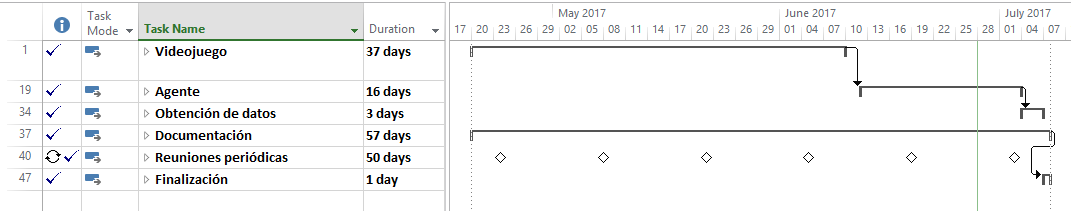
\includegraphics[width=19cm]{otros/capturasPlanificacion/general.PNG}}
	\caption{Cronograma general del proyecto}
	\label{plan:general}
\end{figure}

\subsection{Planificación del videojuego}

\begin{figure}
	\centerline{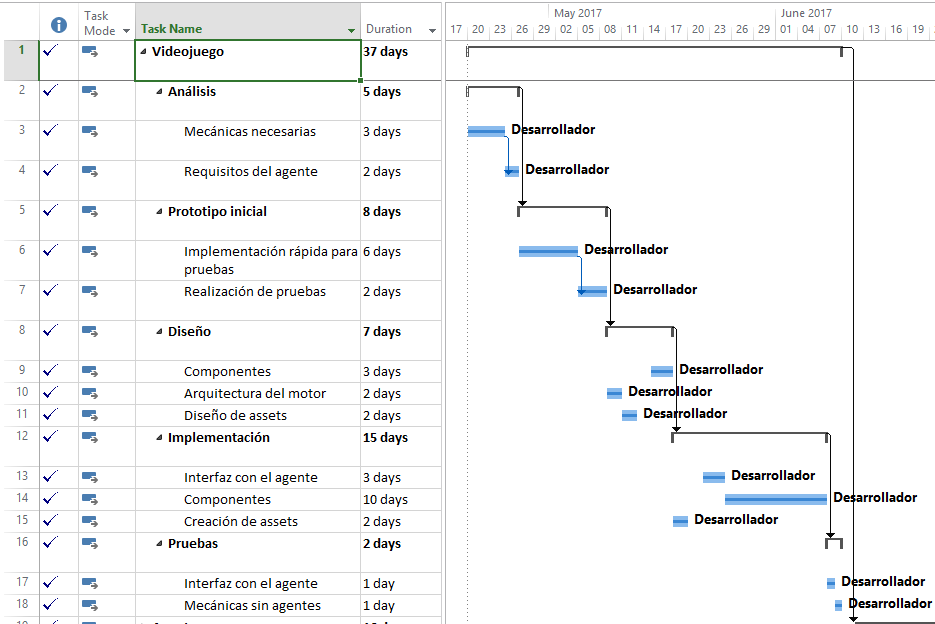
\includegraphics[width=19cm]{otros/capturasPlanificacion/videojuego.PNG}}
	\caption{Cronograma de la parte del videojuego}
	\label{plan:videojuego}
\end{figure}

En la figura \ref{plan:videojuego} se puede observar un desglose de las tareas correspondientes a la creación del videojuego en todos los sentidos. Se comienza por una etapa de análisis en la que se intenta diseminar cuales son las \textbf{mecánicas} que se necesitarán implementar para dar una experiencia jugable lo suficientemente buena para luego centrarse en descubrir que \textbf{requisitos} puede que necesite la aplicación para acomodar al agente que luego se añadirá.

\bigskip

Seguido de esto se encuentra el apartado que forzó a rehacer parte de la planificación y que se relaciona estrechamente con el riesgo RSK-9 (Imposibilidad de realizar simulaciones aceleradas). Fue durante la ejecución de la tarea de \textbf{pruebas} en la cual se descubrió que la \textbf{implementación} con la tecnología anterior no podía cumplir los requisitos del proyecto.

\bigskip

La acción correctiva AC-1 para el riesgo RSK-9 hizo que fuera necesario agregar tareas de \textbf{diseño de componentes} y \textbf{diseño de arquitectura del motor} a la ya existente tarea de \textbf{diseño de \textit{assets}}. Una vez terminada esta etapa de diseno se procede a la implementación de acuerdo con lo definido en la etapa anterior, esta etapa contiene la tarea más larga del proyecto al ser necesario \textbf{implementar los componentes} del motor desde cero, además de crear la \textbf{interfaz con el agente} y realizar la \textbf{creación de \textit{assets}} que implicaría dibujar las animaciones, generar los sonidos, etc.

\bigskip

Finalmente se realizan una serie de tareas dedicadas a pruebas en las que se comprueba el correcto funcionamiento de la posible interfaz con el futuro agente y las mecánicas generales del juego cuando aún no se ha añadido dicho agente.


\subsection{Planificación del agente}

\begin{figure}
	\centerline{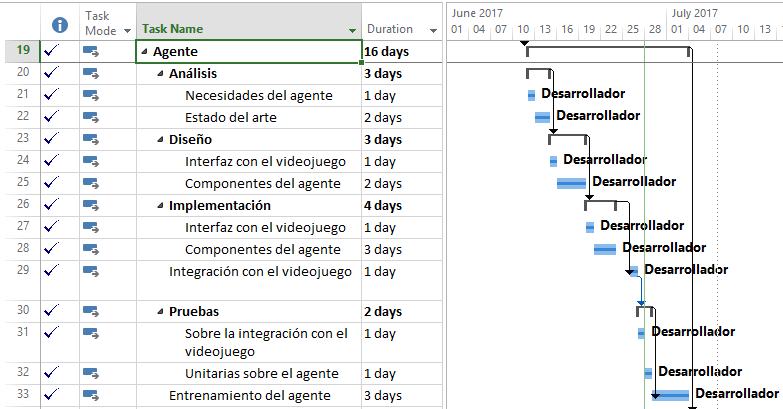
\includegraphics[width=19cm]{otros/capturasPlanificacion/agente.PNG}}
	\caption{Cronograma de la parte del agente}
	\label{plan:agente}
\end{figure}

Se dedica ahora este apartado a explicar la figura \ref{plan:agente} que contiene la planificación asociada a todas las etapas que contienen las tareas que darán lugar al agente final. Es importante comentar que la duración de esta etapa había sido planificada de forma que era significativamente más larga. Sin embargo, la AC-1 hizo que se alargada más de lo inicialmente esperado la etapa dedicada al videojuego y redujo el tiempo disponible para el agente.


\bigskip

Se comienza, como era de esperar, por una etapa de \textbf{análisis} que nos ayudaría a obtener la información necesaria sobre lo que necesitaríamos para realizar una buena implementación, ya sea en forma de requisitos, riesgos que se deben considerar, etc. Primero se analizan las \textbf{necesidades de nuestro agente} dependiendo del juego para juego investigar el \textbf{estado del arte} para ver que información nos puede ser útil.

\bigskip

Dentro de las etapas de \textbf{diseño e implementación} se incorporan tareas dedicadas a definir e implementar tanto una \textbf{interfaz con el videojuego} creado como los \textbf{componentes} necesarios para que el agente funcione. Luego de estas dos etapas se realiza una \textbf{integración con el videojuego}.

\bigskip

Una vez que la aplicación está integrada se necesita hacer una serie de \textbf{pruebas} sobre dicha \textbf{integración} para ver que ambas interfaces cumplen su función. Además de eso, para comprobar el buen funcionamiento del agente se realizan una serie de pruebas \textbf{unitarias} sobre el mismo. Una vez superadas las pruebas se puede proceder a \textbf{entregar} al agente mediante la iteración de simulaciones que permite la aplicación.


\subsection{Planificación de la obtención de datos}

\begin{figure}
	\centerline{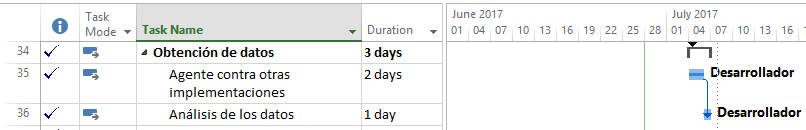
\includegraphics[width=19cm]{otros/capturasPlanificacion/obtencion_de_datos.PNG}}
	\caption{Cronograma de la parte de obtención de datos}
	\label{plan:datos}
\end{figure}


Esta pequeña sección contiene explica las tareas presentes en la figura \ref{plan:datos}. La primera tarea consiste en \textbf{probar al agente} una vez realizadas las tareas de aprendizaje. Para este fin se usa una implementación basada en reglas creada por el desarrollador y utilizando su conocimiento experto en el videojuego para comprobar como el agente es capaz de comportarse.

Se obtendrán datos sobre como se comporta con distintos niveles de entrenamiento y realizando diferente número de simulaciones, contra el mismo y contra el enemigo basado en reglas. Finalmente, los datos obtenidos se procesarán en la tarea de \textbf{análisis de datos}.


\subsection{Planificación de la documentación, reuniones y finalización}

\begin{figure}
	\centerline{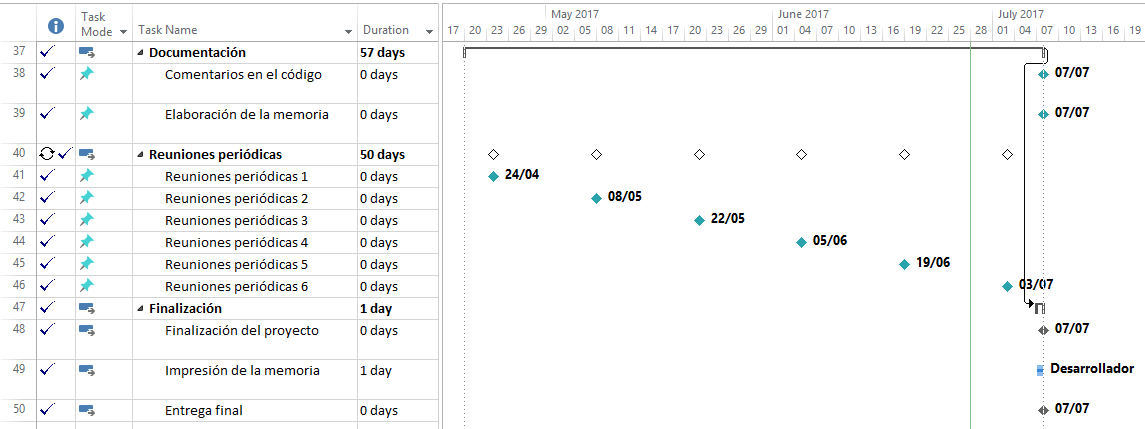
\includegraphics[width=19cm]{otros/capturasPlanificacion/documentacion_reuniones_final.PNG}}
	\caption{Cronograma de la parte de documentación, reuniones y finalización}
	\label{plan:fin}
\end{figure}

Por último, en este apartado se pueden ver las tareas de primer nivel dedicadas a la \textbf{documentación}, las\textbf{reuniones} y la \textbf{finalización} del proyecto.

\bigskip

Sobre la documentación hay que comentar que tanto la tarea de \textbf{comentarios en el código} como la de \textbf{elaboración de la memoria} se ha introducido una duración nula pues se han llevado a cabo con todas las otras tareas del proyecto. Esta es la razón por la cual se ha introducido la tarea de documentación en si misma como una tarea \textit{hamaca} de todo el proyecto\footnote{Una tarea hamaca es aquella cuya duración depende de cuando empiezan y terminan otras tareas del proyecto.}. Si se introdujera una duración específica se estaría duplicando el trabajo en la planificación pues esas horas ya se han tenido en cuenta en las otras tareas del proyecto.

\bigskip

En lo que a las \textbf{reuniones periódicas} se refiere, se ha agregado una tarea recursiva que indica cuando se realizaron las reuniones con los tutores. Su duración, de un modo similar a las tareas de documentación, es nula porque el tiempo empleado se tiene en cuenta en las otras tareas. Si se le fuera a asociar una duración se tendría que hacer en términos de horas pues no se dedicaba todo un día a realizar una reunión. Utilizar horas en lugar de días suele ser un síntoma de haber desgranado las tareas demasiado y se considera mala práctica por cierta parte de la comunidad de gestión de proyectos.

\bigskip

Finalmente se agregan las tareas relacionadas con la \textbf{finalización} del proyecto, marcando un hito para dicha finalización, dedicando un día a \textbf{imprimir y comprobar la memoria} y dejando el último día como hito para realizar la \textbf{entrega final}.



\section{Análisis de costes}

Este apartado estará dedicado a realizar un análisis de los costes asociados al proyecto con el objetivo de generar un presupuesto que nos permita controlar los gastos. Los tipos de costes que se considerarán son los siguientes:

\begin{itemize}
	\item \textbf{Directos}: Los que de identifican claramente como costes definidos para el proyecto, un buen ejemplo es la compra de software o el pago por horas trabajadas.
	\item \textbf{Indirectos}: El PMBOK\cite{pmbok} ayuda a identificar los costes indirectos como aquellos que no se pueden asignar de forma directa a un proyecto concreto. Por esta razón se acumulan y distribuyen equitativamente entre diferentes proyectos mediante un procedimiento específico.
\end{itemize}

Pese a que el proyecto sea realizado en un ámbito académico por solamente un alumno no se debe restar importancia a este apartado ya que una buena gestión de costes es vital para que un proyecto salga adelante. Un buen ejemplo nos lo da el Chaos Report\cite{chaos} que indica que recientemente el 50.7\% de los proyectos de software cuestan una media del 189\% más de lo esperado y que el 31.1\% de todos los proyectos se cancelarán antes de ser completados. Otro dato preocupante es el que indica que solo el 15.5\% de la totalidad de proyectos evaluados está por debajo de un 20\% de coste adicional.

\bigskip

Continuando ahora con el análisis de costes directos se ve que, al haber priorizado la utilización de software libre o versiones de prueba, los elementos a tener en cuenta son muy reducidos.

\bigskip 

El más importante de los mismos es el salario del desarrollador para lo cual se ha investigado el valor medio pagado a un analista programador en Galicia. Dicha información se ha obtenido de un estudio salarial realizado por la consultoría Vitae\cite{vitae}  del cual se obtiene que el valor medio para un analista-programador junior de C++ es de 16000\euro{} brutos anuales. A raíz de datos que se nos han proporcionado durante los estudios en la asignatura de Gestión de Proyectos obtenemos que los impuestos suman los siguientes porcentajes: 

\begin{itemize}
	\item 5.5\% de Seguridad Social
	\item 23.6\% de Contingencias Comunes
	\item 0.2\% de FOGASA
	\item 0.7\% de Formación Profesional
\end{itemize}

Lo que corresponde a un incremento total del 30\% sobre el salario bruto que genera en la tabla \ref{tab:salario} con los valores que nos llevan al coste/hora final.

\begin{table}
		\begin{tabular}{|l|l|l|l|l|}
			\hline
			\textbf{Bruto anual} & \textbf{Impuestos} & \textbf{Total anual} & \textbf{Total mensual} & \textbf{Coste/hora} \\
			
			\hline
			16000\euro{}& 4800\euro{} & 20800\euro{} & 1486\euro{} & 9.30\euro{} \\
			
			\hline
		\end{tabular}
		\caption{Tabla de salario del desarrollador}
		\label{tab:salario}
\end{table}

\bigskip

Otro de los costes directos a considerar será el precio de impresión de la memoria y los materiales necesarios para crear el proyecto en formato CD. Teniendo en cuenta una longitud cercana a las 150 páginas y el precio de la grabación del CD se agregarán 100\euro{} en concepto de ambos aspectos.

\bigskip

Considerando ahora los costes indirectos agregaremos el coste de amortización relacionado al equipo de desarrollo utilizado. El MacBook Pro utilizado costó en su día 2923,36\euro{} y se le estimará una vida media de unos 5 años (60 meses). Dado que el proyecto se extendió aproximadamente 3 meses obtenemos los datos de la tabla \ref{tab:mac}.

\begin{table}
	\begin{tabular}{|l|l|l|l|}
		\hline
		\textbf{Meses de vida} & \textbf{Meses de utilización} & \textbf{Coste total} & \textbf{Coste en el proyecto}\\
		
		\hline
		60{}& 4{} & 2923,36\euro{} & 194.90\euro{} \\
		
		\hline
	\end{tabular}
	\caption{Tabla de costes de amortización del equipo}
	\label{tab:mac}
\end{table}

\bigskip

Finalmente sumaremos un 10\% al sobre el coste del proyecto en concepto de gastos en servicios como electricidad, agua, internet, etc. Teniendo en cuenta el pago final\footnote{Considerando 14 pagas, 20 días laborales al mes con 8 horas de trabajo al día.} al desarrollador con el resto de gastos directos e indirectos se obtienen los datos de la tabla \ref{tab:coste_final}.


\begin{table}
	\begin{center}
	\begin{tabular}{|l|l|}
		\hline
		\textbf{Elemento} & \textbf{Coste (\euro{})}\\
		
		\hline
		Analista programador C++ & 3952.50 \\
		\hline
		Amortización del equipo & 194.90 \\
		
		\hline
		Xcode 9& 0 \\
		
		\hline
		Unity 5& 0 \\
		
		\hline
		Clang 4& 0 \\
		
		\hline
		Audacity 2.1.3 & 0\\
		
		\hline
		StarUML 2& 0 \\
		
		\hline
		Atom 1.19& 0 \\
		
		\hline
		Microsoft Project 2013& 0 \\
		
		\hline
		TeXstudio& 0\\
		
		\hline
		Impresión memoria + CD & 100 \\
		
		\hline
		GraphicsGale 2.06& 0 \\
		
		\hline
		Dropbox& 0 \\
		
		\hline
		Google Drive& 0 \\
		
		\hline
		Git \& GitHub& 0 \\
		
		\hline
		Costes indirectos& 10\% (424.74) \\
		
		\hline
		\textbf{TOTAL: } & 4672.14 \\
		
		\hline
	\end{tabular}
	\caption{Tabla de costes finales}
	\label{tab:coste_final}
	\end{center}
\end{table}

\clearpage

\section{Plan de Gestión de las Comunicaciones}

\todo{Completar el plan de Gestión de las Comunicaciones}